
%(BEGIN_QUESTION)
% Copyright 2015, Tony R. Kuphaldt, released under the Creative Commons Attribution License (v 1.0)
% This means you may do almost anything with this work of mine, so long as you give me proper credit

This production process manufactures {\it ammonium nitrate}, a principal ingredient of synthetic fertilizer, from the chemical combination of nitric acid and ammonia:

$$\includegraphics[width=15.5cm]{i0008rx01.eps}$$

Examine the level control system for the rundown tank (V-7), and identify one of the loads in that control loop.  After identifying the load, add a transmitter to sense that load variable, and add necessary control functions to implement a {\it feedforward} control strategy to the rundown tank's level control.

\underbar{file i01276}
%(END_QUESTION)





%(BEGIN_ANSWER)

Perhaps the most significant load on the rundown tank's level control loop is the incoming flow rate from the neutralizer vessel (V-6) through the line with the three pH transmitters, since any changes in this flow rate will cause the level controller (LIC-26) to take corrective action to maintain level at setpoint.

\vskip 10pt

The feedforward transmitter for this load, of course, will be a flow transmitter added to the line carrying ammonium nitrate from V-6 to V-7.  This transmitter's signal will pass through a gain/bias function and then (possibly) through a lead/lag function before entering a summer function placed between LIC-26 and FIC-25.  This way, the proportioned feedforward signal will be added to the cascaded setpoint of FIC-25 calling for more or less discharge flow from V-7 in accordance with the amount of flow entering V-7 from V-6.
 
%(END_ANSWER)





%(BEGIN_NOTES)


%INDEX% Control, strategies: feedforward
%INDEX% Process: ammonium nitrate production (realistic P&ID shown)

%(END_NOTES)


